\documentclass[10pt, notitlepage,a4paper]{article}
\usepackage[margin=0.9in]{geometry}
\usepackage[T1]{fontenc}
\usepackage[utf8]{inputenc}
\usepackage[english, polish]{babel}
\let\babellll\lll
\let\lll\relax
\usepackage{amssymb,url}
\usepackage{ntheorem,tikz}
\usepackage{graphicx,lmodern}
\newcommand*\ruleline[1]{\par\noindent\raisebox{.8ex}{\makebox[\linewidth]{\hrulefill\hspace{1ex}\raisebox{-.8ex}{#1}\hspace{1ex}\hrulefill}}}
\usetikzlibrary{calc,matrix,arrows}
\usepackage{algorithmicx,algorithm}
\usepackage{fixltx2e}
\usepackage[noend]{algpseudocode}
\MakeRobust{\Call}
\pagestyle{empty}
%----------------------Marginesy------------
\setlength{\parindent}{0mm}
\setlength{\parskip}{2mm}

\newcommand{\N}{\mathbb{N}}
\newcommand{\xdotminus}[2]{%
  \ooalign{\hidewidth$\vcenter{\hbox{$#1\dot{}$}}$\hidewidth\cr$#1-$\cr}%
}
\providecommand{\dotminus}{\mathbin{\mathpalette\xdotminus\relax}}

%%%%%%%%%%%%%%%%%%
\theoremheaderfont{\normalfont\bfseries}
\theoremseparator{.}
\theorembodyfont{\normalfont\upshape}
\theoremstyle{plain}

\theoremindent1em
\newtheorem{zadanie}{Zadanie \hspace{-0.4em}}

\newtheorem{zadanieW}{Zadanie W\hspace{-0.4em}}  

% Długa lista więc dam numery stron
\pagestyle{plain}


\begin{document}
\section*{Podstawowy warsztat informatyka --- lista 6}
\begin{zadanie} (0 punktów) 
Wejdź na stronę \url{http://learngitbranching.js.org} i ukończ tutorial w zakresie zakładki main oraz Push \& Pull -- Git Remotes! z zakładki Remote.
\end{zadanie}

\begin{zadanie} (4+2* punkty) 
Wejdź na stronę \url{http://learngitbranching.js.org/?NODEMO}. Stwórz repozytoria w takich kształtach, jak na załączniku do tej listy (kolory nie muszą się zgadzać, nie martw się też, jeśli ścieżki się inaczej ułożą). Każde repozytorium jest warte 2 punkty.
\end{zadanie}

\begin{zadanie} (3 punkty) Będziemy tworzyć i łączyć gałęzie.
\begin{itemize} 
\item 
Stwórz puste repozytorium gita.
Utwórz w nim plik \verb+README.md+ o treści ,,Zadanie 3 z listy 6 z PWI''. Skomituj ten plik (do gałęzi \verb+master+).

\item Utwórz w tym repozytorium gałąź \verb+ja+. Utwórz plik tekstowy \verb+o-mnie.txt+ i umieść w nim swoje imię i nazwisko. Zmiany te skomituj do gałęzi \verb+ja+.

\item Zastanów się, jaka jest najciekawsza rzecz, którą dotychczas poznałaś/poznałeś na naszych studiach. Dopisz tę informację (w nowej linii) do pliku \verb+o-mnie.txt+ i ponownie skomituj zmiany.

\item W kolejnej linii wpisz nazwę jakiegoś podcastu lub kanału, który subskrybujesz. Znów skomituj zmiany. W tym momencie repozytorium powinno się składać z trzech komitów w gałęzi \verb+ja+. 

\item  Wróć do gałęzi \verb+master+. Utwórz nową gałąź \verb+komputer+. Utwórz w niej plik \verb+o-komputerze.txt+ zawierający wynik polecenia \verb+uname -a+. Skomituj ten plik. Następnie doklej do niego zawartość \verb+/proc/meminfo+ i znowu skomituj.

\item Wróć do gałęzi \verb+master+. Dopisz coś do pliku \verb+README.md+ i skomituj zmiany. Obejrzyj wyniki poleceń  \verb+git log+, \verb+git reflog+ oraz \verb+gitk+. W \verb+gitk+ utwórz widok zawierający wszystkie gałęzie.

\item Wróć do gałęzi \verb+ja+ i dodaj tam plik \verb+ulubiony-film+ zawierający nazwę Twojego ulubionego filmu, a następnie skomituj te zmiany.

\item Ojej, zapomniałem napisać, że w komicie dotyczącym czasopisma trzeba było dodać jeszcze linię z nazwą Twojego ulubionego koloru! Trzeba to poprawić. Wykorzystaj polecenia \verb+git rebase+ oraz \verb+git commit --amend+, aby to zrobić. Następnie poukładaj komity tak, jak były.

\item Przejdź do gałęzi \verb+master+ i dodaj do niej komity dotyczące pliku \verb+o-mnie.txt+ z gałęzi \verb+ja+ poleceniem \verb+git cherry-pick+. Następnie dołącz gałąź \verb+komputer+ poleceniem \verb+git merge+.

\item Przejdź do komita (nie gałęzi!), w którym stworzyłeś plik \verb+ulubiony-film.txt+. Dopisz do niego rok wydania tego filmu, a następnie skomituj zmiany. Dodaj tag do tego komita. Przejdź do gałęzi \verb+master+ i zrób \verb+merge+ z otagowanym komitem. 

%\item (1 punkt) Stwórz swoje repozytorium klikając odpowiedni odnośnik poniżej, a następnie umieść tam efekty swojej pracy (całe repozytorium ze wszystkimi gałęziami).
%Otwórz to repozytorium w przeglądarce i pokaż prowadzącemu.
%\url{https://classroom.github.com/a/v05qfM2w}
\end{itemize}
\end{zadanie}

\begin{zadanie}{(3 punkty)} 
Stwórz swoje repozytorium robocze pod adresem:

\begin{center}
\url{https://classroom.github.com/a/ma-LJSGa}
\end{center}

Ściągnij to repozytorium na dysk. Zwróć uwagę, że ma ono dwie gałęzie -- w gałęzi master jest plik \verb+przyklad.tex+, a w gałęzi main tylko .gitignore (na razie nie musisz wiedzieć, co ten plik robi, ale on jest tam, by pomagać studentom).

Spraw, by w gałęzi main pojawił się plik \verb+sprawozdanie.tex+ o treści identycznej z \verb+przyklad.tex+.

Skompiluj plik \verb+sprawozdanie.tex+ jeden raz. Zrób kopię otrzymanego pliku pdf, a następnie skompiluj drugi raz -- czy widzisz różnicę?

Nie dodawaj żadnych plików utworzonych przez kompilator do repozytorium!

W pliku \verb+sprawozdanie.tex+  usuń wszystko pomiędzy \verb+\begin{document}+ a \verb+\end{document}+. Spróbuj testowo wpisać tam własny tekst, a następnie skompilować ten plik. Upewnij się, że edytujesz go we właściwym kodowaniu (domyślnie UTF-8). 

Zmień dane osobowe w pliku \verb+sprawozdanie.tex+ na swoje oraz dodaj polecenie  \verb+\maketitle+ zaraz po \verb+\begin{document}+. 
Utwórz pięć rozdziałów (ang. section) opisanych poniżej. Po każdym rozdziale rób \verb+commit+ i \verb+push+.
\begin{itemize}
\item  W pierwszym rozdziale wytłumacz własnymi słowami, co zwraca polecenie \verb+id+. Opis powinien być zrozumiały dla osób, które mają mgliste pojęcie o systemie Linux.
\item Przed napisaniem drugiego rozdziału dowiedz się, co to jest czas uniksowy (zwany również czasem POSIX). Następnie opisz, na czym polega problem roku 2038. Do swoich danych osobowych (umieszczonych wewnątrz \verb+\author{}+) dopisz, po przecinku, swoją datę urodzenia zapisaną w czasie uniksowym (możesz wybrać dowolną godzinę tego dnia).
\item W kolejnym rozdziale opisz własnymi słowami, z czego wynikała różnica pomiędzy plikiem przykładowym skompilowanym raz, a skompilowanym dwa razy.
\item W czwartym rozdziale wyjaśnij, dlaczego suma ciągu $1$, $\frac{1}{2}$, $\frac{1}{4}$, $\dots$ wynosi $2$.
\item W ostatnim rozdziale wstaw swoje ulubione zwierzątko w ASCII art. Zwierzątko możesz znaleźć na Google, trudnością w tym zadaniu będzie zadbanie o to, by zwierzątko się nie ,,rozjechało''.
{\tiny
\begin{verbatim}
                                      _.--"""--,
                                    .'          `\
  .-""""""-.                      .'              |
 /          '.                   /            .-._/
|             `.                |             |
 \              \          .-._ |          _   \
  `""'-.         \_.-.     \   `          ( \__/
        |             )     '=.       .,   \  
       /             (         \     /  \  /
     /`               `\        |   /    `'
     '..-`\        _.-. `\ _.__/   .=.
          |  _    / \  '.-`    `-.'  /
          \_/ |  |   './ _     _  \.'
               '-'    | /       \ |  
                      |  .-. .-.  |
                      \ / o| |o \ /
                       |   / \   |
                      / `"`   `"` \
                     /             \
                    | '._.'         \
                    |  /             |
                     \ |             |
                      ||    _    _   /
                      /|\  (_\  /_) /
              jgs     \ \'._  ` '_.'
                       `""` `"""` 
\end{verbatim}
}
\end{itemize}
\end{zadanie}

\begin{zadanie}{(4* punkty)}
Stwórz swoje cv w \LaTeX{}u, pracując w repozytorium założonym pod adresem \url{https://classroom.github.com/a/-kH1H4_2}. Powinno mieć długość 1 lub 2 stron i~spełniać wszystkie standardy (dla przykładu, powinno zawierać klauzulę o zgodzie na przetwarzanie danych). Rozwiązania należy przesłać najpóźniej 21.12 o 14:15.
\end{zadanie}
\newpage
\section*{Załącznik}
\section{Scalenie ścieżek}
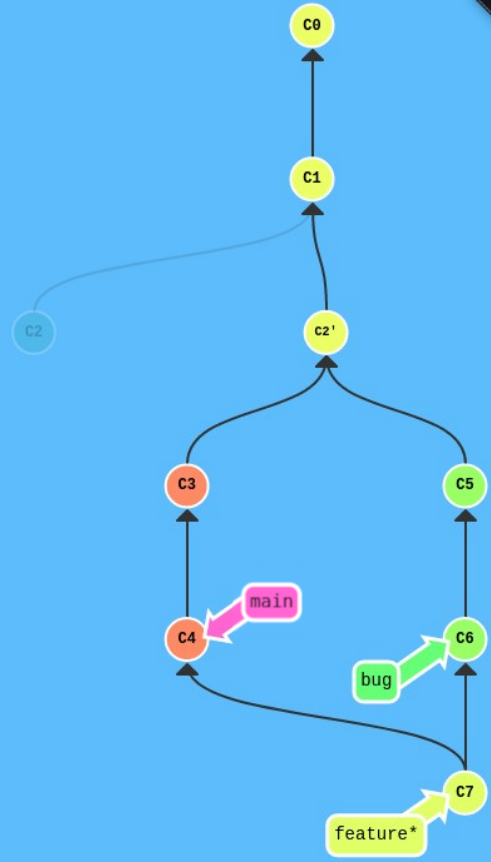
\includegraphics[scale=0.45]{pics/830.png}

\section{Bardziej skomplikowany przykład z oderwaną głową}
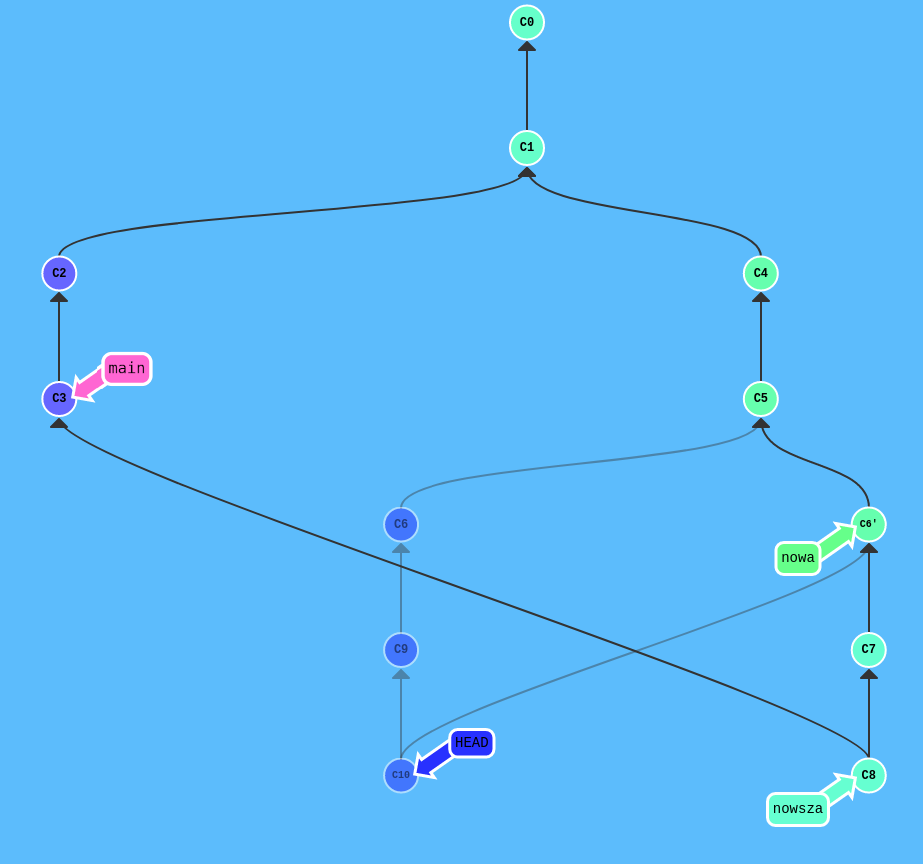
\includegraphics[scale=0.5]{pics/merge.png}

\section{Repozytorium z clone za bonusowy punkt}
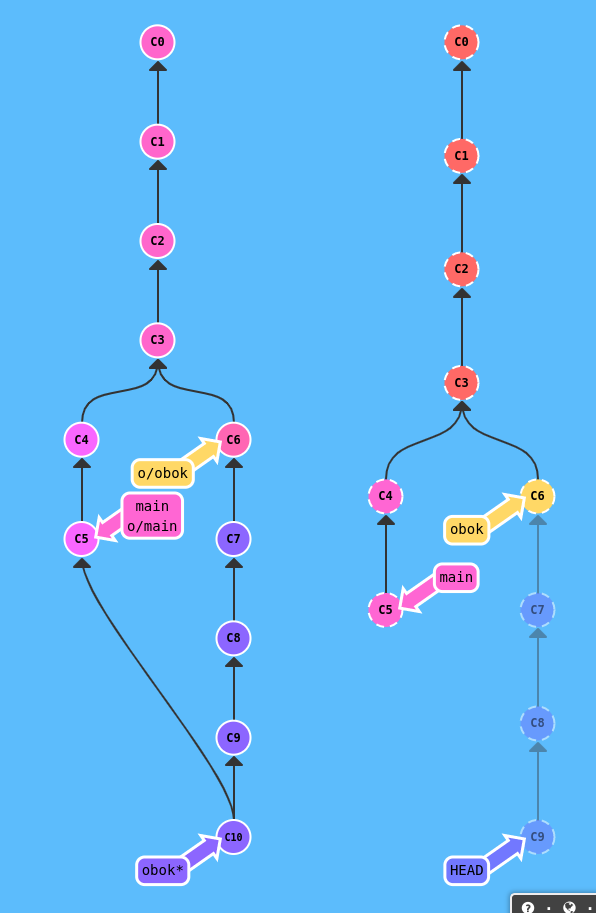
\includegraphics[scale=0.5]{pics/clone.png}


\end{document}